\chapter{Introduction}

%\RC{Not sure that in general this is the economic goal of society. Maybe more like a capitalistic society? Or free-market? Probably should double check and clarify this point.}

An economic goal of a capitalistic society is to maximize wealth by allocating resources efficiently.  Capital markets (such as the stock market) provide a method to help allocate resources efficiently. As a result, the prediction and inference of future financial events within a capital market are often critical to achieving the economic goal. Since firm-specific information contributes to resource allocation (i.e., labor, capital, and natural resources) in capital markets, the prediction of a future state for a firm (such as its profitability, financial condition, or revenue growth) is an essential factor contributing to resource allocation.  In this introduction, we review several different methods that can be used to predict or inform about the future state of a firm.  


\section{Machine Learning}

Machine Learning encompasses a vast set of statistical tools for understanding data and making predictions and inferences. These tools fall into supervised or unsupervised categories. For data-driven problems, typically, we have a response variable (or labels)  referred to as \(Y\), and \(p\) independent variables (or features) referred to as \(X\). Given the assumption that there is some relationship between \(Y\) and \(X\) the relationship can be expressed as:

\begin{equation}
\label{eq:function}
Y = f(X) + \epsilon
\end{equation}

\noindent In Equation \ref{eq:function} \(f\) is an unknown function that models the relationship between \(X\) and \(Y\) with  \( \epsilon \) noise.  In most cases, it is not possible to perfectly model \(f\) with real-world data, so we instead estimate the function \(f\) by an estimator (\(\hat{f}\)). If \(Y\) is a quantitative variable in Equation\ref{eq:function}, we use regression techniques to estimate \(f\); however, if \(Y\) is a qualitative variable, we use classification techniques instead.   \(\hat{f}\) is sought for inference where one wants to estimate \(f\) to understand how \(\hat{Y}\) (predicted labels) changes as one adjusts features. \(\hat{f}\) is also sought for prediction where the only concern is the accuracy of predictions for \(Y\). Machine learning provides a variety of approaches to estimate \(f\) for prediction and inference (see, \eg \cite{ISL}).

Machine learning problems typically fall into either supervised learning, semi-supervised learning, or unsupervised learning. With supervised learning, one wants to fit a model on labels using a set of features. Semi-supervised learning consists of a domain with features where only a subset have corresponding labels. Typically, in this setting, one wishes to use the given features and partial labels to determine the remaining missing labels. Lastly, with unsupervised learning, one has features and no associated labels and seeks to find structure between the features.  In this dissertation, the presented results will only utilize supervised learning. 

\subsection{Supervised Learning} \label{sec:SupervisedLearning}
In a supervised learning paradigm, it is not enough to only have \(\hat{f}\) estimate \(f\) well on a dataset. Instead, we seek to estimate \(\hat{f}\) sufficiently well so that this estimator will also perform well on new data that  \(\hat{f}\) has not seen before. To find a suitable \(\hat{f}\), a standard methodology is to partition the data into a training set and testing set (see Figure \ref{fig:TrainTestSplit}). The training set consists of data to train the model. The testing set consists of data to assess \(\hat{f}\)'s ability to generalize well to new data. The researcher/practitioner typically determines the ratio of data used to train and assess the model.  A specific  \footnote{One can use many error metrics; however, for the sake of brevity MSE is the only error metric discussed.}  way to estimate  \(\hat{f}\)'s performance for a regression model is to use an error metric such as mean squared error (MSE) given by:  

\begin{equation}
\label{eq:MSE}
MSE = \frac{1}{n} \sum_{i=1}^n (y_i -\hat{f}(x_i))^2
\end{equation}

\noindent In Equation  \ref{eq:MSE}, \(y_i\) and \(x_i\) are the \(i^{th}\) observations of the labels and features respectively. \(\hat{f}(x_i)\) is the prediction of \(\hat{f}\) for the \(i^{th}\) observation and \(y_i\) is the label for the \(i^{th}\) observations. Training MSE indicates the mean standard error of the estimator's ability to learn the training data.  Subsequently, there is a testing MSE associated with the mean standard error of the estimator on the withheld testing data. A model with a small testing MSE often generalizes well to the withheld data. Often, the training MSE and testing MSE differ where the training MSE underestimates the MSE for the testing MSE (see chapter 5 of \cite{ISL}). Given the importance of this task, a number of approaches have been developed that can produce a more accurate estimate of how well \(\hat{f}\) will generalize to new data.

\subsection{Validation Approaches} \label{sec:validationApproach}

An alternative approach to training and assessing \(\hat{f}\) on training and testing sets, respectively, is to create a validation dataset by randomly sampling the training dataset.  The researcher/practitioner determines the sampling method.  \(\hat{f}\) trains on the training data, and the trained model assesses its ability to generalize with validation data. The validation MSE is more indicative of the test MSE. However, there are issues with this approach. For example, randomly sampled data is in the validation dataset.  Given that the validation set is composed of random data, the validation MSE can be highly variable. A generally accepted solution to reducing the variability of the validation MSE is cross-validation.

A common cross-validation technique is \(k\)-fold cross-validation where the training data is split into \(k\) separate folds (see Figure \ref{fig:KFoldValidation}). The first fold is withheld and used as the validation dataset to assess the model's performance. The remaining \(k-1\) folds train the model. For the next iteration, the same procedure repeats where the second fold serves as the validation dataset to assess the model (see Figure \ref{fig:KFoldValidationExplain}) and the other \(k-1\) folds train the model. This process repeats \(k\) times and  produces \(k\) \(MSE\) scores (\(MSE_1, MSE_2, ... , MSE_k\)). Averaging the MSE fold values yields the \(k\)-fold CV estimate:

\begin{equation}
\label{eq:CV}
CV = \frac{1}{k} \sum_{i=1}^k MSE_i
\end{equation}

\noindent where \(k\) is the number of folds. 

Selecting a large value \(k\) can be computationally expensive as the model must be retrained on \(k\) different folds. In addition to this, the selection of \(k\) can affect the model's ability to generalize to new data well. Typically with a smaller value of \(k\) you have more bias, and a larger value of \(k\) has more variance. For example consider when \(k=3\) and \(k=10\), the training folds will have \(n_{train}\) observations where  \( n_{train}= \frac{(k-1)n}{k}\) and the validation fold will have \(n_{validation}\) observations where \( n_{validation}= \frac{k-(k-1)n}{k}\). When \(k=10\), 90\% of the data is used to train the model, and the remaining 10\% assesses the model. The model trains on very similar datasets, and the predictions from the model on the cross-validation datasets are highly correlated. The highly correlated datasets can produce a model with a high variance. If \(k=3\) 66.7\% of the data trains the model and the remaining 33.3\% of the data assesses the model. In this case, cross-validation averages fewer predictions that are less correlated with each other since the overlap between the training sets are smaller. When \(k=3\) this results in a CV score with lower variance, but since each model is trained on a smaller set of the original training data there is potential for a higher bias. 

% wrap ML up.

\section{Network Science} \label{sec:NetworkScience}

% context to how network science is used in Finanical Markets

Network science is the study of networks, and a network (or graph) consists of a collection of nodes joined by connections (commonly referred to as edges).  Networks capture interactions between nodes, and over the years, scientists have discovered that specific patterns of interactions have a significant effect on the network's behavior (see \cite{Networks}.  This field has evolved, and a vast set of tools have been developed to analyze,  model,  and understand networks (again, see \cite{Networks}).  Researchers have used networks in financial markets to determine which market sectors are related around specific events.  For example,   \cite{Billio2012} and \cite{DieboldYilmaz2014}  found that banks play an essential role in transmitting shocks relative to the remaining set of financial firms,  consistent with banks playing a more central role in systemic risk for the economy around the 2007-2009 financial crisis.  Thus, network science can help us  understand more about the probable future states of firms.

Networks can be formed from data to offer an alternative representation of the data, allowing many new analysis techniques. Network Theory involves the study of networks as a representation of relationships between nodes. Throughout this section, \(G\) denotes a network, \(m\) denotes the number of edges in a network, and \(n\) denotes the number of nodes.  A graph with \(n\) nodes and \(m\) edges is denoted as \(G(n,m)\).

Undirected graphs do not have to specify the direction of an edge.  For example, if Node \(A\) and Node \(B\) are connected, an undirected graph will not distinguish whether Node "A" connects to Node "B" or vice-versa;  an undirected graph will only retain information about nodes \(A\) and \(B\) having a connection. Figure \ref{fig:IntroExampleNetwork} shows an example of an undirected graph \(G(7,16)\). The number of edges (or connections to other nodes) a particular node has is known as the degree of the node. Figure \ref{fig:IntroExampleNetwork}, the node "FB" has a degree of six because it connects to six other nodes. Degree is a standard metric used in network theory.

It is also possible for a graph to retain additional information about edges. Another source of information is the direction of the edges; graphs that store information about edges' directions are called directed graphs.  For example,  consider a directed graph with two nodes (Node "A" and Node "B"). If Node "A"  connects to Node "B" a directed graph would contain information that Node "A"  has an edge to Node "B" but Node "B" does not have an edge to Node "A".  Figure \ref{fig:ExampleNetworkDirected} shows an example of a directed graph; in Figure \ref{fig:ExampleNetworkDirected} there is an edge from "JNJ" to "FB"  however there is no edge from "FB" to "JNJ".

Weighted networks (or weighted graphs) assign weights to the edges in a network. Instead of having a binary connection to determine whether an edge is present or not, the weight can provide a measure of the strength between the connections among different nodes. For example, if one has an attribute to determine the strength between nodes, such as a statistic from the data,  it can be used as the weight value of an edge to determine the strength of the connection between those nodes.  Edge weights are applicable to both directed and undirected graphs. Ergo it is possible to have an undirected weighted graph or directed weighted graph. Figure \ref{fig:ExampleNetworkDirectedWeighted} provides an example of a directed weighted network. 

Under certain circumstances, it is more convenient to express a graph as an adjacency matrix.  The graph in Figure \ref{fig:IntroExampleNetwork}, is converted to a table with column and row headers  in Table~\ref{tab:ExampleTable}. However, it is mathematically more convenient to express Table~ \ref{tab:ExampleTable} as an adjacency matrix $A$ (see Equation \ref{eq:adjacencyMatrix}).

\begin{gather}
A =
 \begin{bmatrix}
    0 & 1 & 1 & 1 & 0 & 1 & 1 \\
    1 & 0 & 1 & 1 & 0 & 1 & 1 \\
    1 & 1 & 0 & 1 & 1 & 0 & 0 \\
    1 & 1 & 1 & 0 & 1 & 1 & 1 \\
    0 & 0 & 1 & 1 & 0 & 0 & 0 \\ 
    1 & 1 & 0 & 1 & 0 & 0 & 1 \\ 
    1 & 1 & 0 & 1 & 0 & 1 & 0 \\
  \end{bmatrix}
  \label{eq:adjacencyMatrix}
\end{gather}

\noindent Similar to Table \ref{tab:ExampleTable}, each element (\(A_{ij}\)) in the adjacency matrix \(A\) is assigned a 1 or 0 based on if there is a connection between a row index (\(i\))  and column index \(j\). Note, the adjacency matrix in Equation \ref{eq:adjacencyMatrix} is symmetric because 
the direction of edges are not taken into account; ergo if node \(i\) and node \(j\) are connected \(A_{ij}\) and \(A_{ji}\) both have a value of 1. This approach can be extended to represent directed graphs by assigning a 1 to a matrix element \(A_{ij}\) where node \(i\) is connected to node \(j\). Lastly, you can express the weight of edges in adjacency matrices by assigning the weight values, which are non-binary, as the matrix elements.

\subsection{Analysis of Networks}
After forming a network from data, common metrics are often sought to help describe the structure of the network.  The first metric is the degree of nodes where the degree  can be defined in Equation \ref{eq:degree} as the sum of edges for a particular node. In Figure \ref{fig:ExampleNetworkDegree}, the node sizes are scaled based on the degree.

\begin{equation}
    \label{eq:degree}
    m_i =  \sum_{ij}A_{ij}
\end{equation}

 \noindent where \(A\) is an adjacency matrix. Subsequently, there are degree measures for directed networks, such as in-degree, which counts the number of edges connected to node \(i\) (see Equation \ref{eq:indegree}), and out-degree, which counts the amount of edges that node \(i\) is connected to (see Equation \ref{eq:outdegree}).

\begin{equation}
    \label{eq:indegree}
    m_i^{in} =  \sum_{j=1}^{n}A_{ij}
\end{equation}

\begin{equation}
    \label{eq:outdegree}
    m_i^{out} =  \sum_{i=1}^{n}A_{ij}
\end{equation}

\noindent The network's density provides a numerical value for the proportion of actual connections out of all potential connections in a network. If all potential connections in a network are present,  the density will have a numerical value of 1, and if there are no connections in an undirected network, the density will be 0. The maximum number of potential connections in a network is \(n(n-1)/2\).  The degree summed for all nodes is \(m\) (for directed networks, the summed in-degree and out-degree for all nodes is \(m\)). The density for a directed graph is:

\begin{equation}
    \label{eq:density}
    D = \frac{m}{n (n-1)}
\end{equation}

Centrality is another metric that is used to measure the importance of individual nodes within a network. Measuring the degree of nodes in relation to other nodes is called degree centrality (see Equation \ref{eq:degreeCentrality}). 

\begin{equation}
    \label{eq:degreeCentrality}
    C_i^d =  m_i = \sum_{ij}A_{ij}
\end{equation}


\section{Information Transfer in Financial Markets} \label{IFinFM}
% Tailor this section such that I dicuss Information Transfer in  a traditional context first, then explain transfer entropy.

The price discovery process plays a vital role in achieving the economic goal for a society.   In particular, how information transfers from one price to another is useful in the price discovery process.  Information is embedded in price, and an efficient market changes rapidly (if not instantaneously) when new information arrives.  For example, Apple Inc. recently announced that their new line of computers (Macs) would use central processing units (CPUs) developed in-house and transition away from Intel CPUs.  This information will rapidly be reflected both in Apple's stock price and Intel's stock price in ideal settings.

In the Apple and Intel example, it is probable that additional information reflects in Intel's price change at a given moment. However, it is difficult to determine price changes for specific events. The entire set of information that reflects in the price change at a given time is unknown.  Prior studies have examined the price changes over long windows such as days or weeks (see \cite{Foster1981} and \cite{Baginiski1987}).  In particular, \cite{Foster1981} measured information transfers from firms that announce earnings and non-announcement firms in the same industry based on short-window price reactions.  Subsequent studies use a similar approach to examine short-window price reactions to firm-level earnings announcements (see \cite{ClinchSinclair1987},   \cite{PownallWaymire1989},  \cite{HanWild1990},  \cite{Wang2014},  and \cite{HannKimZheng2019}).   %The window sizes in the prior works were typically daily.  %These methodologies may have missed much of the price change process given the assumption that information effects the price within seconds.  Given the theory that markets are efficient and reflect information into price within seconds after the information is known,  we seek suitable methods to measure information flow in financial markets.

\subsection{Information Theory } \label{sec:InformationTheory}
Information theory provides a framework for studying the quantification, storage, and communication of information (see \cite{InfoTheoryApplication}).  Information theory has been  shown to be useful in the price discovery process (see \cite{Billio2012} or \cite{DieboldYilmaz2014}), as it offers an alternative approach for understanding the impacts of information on price.   In particular,  it offers alternative methods to understand information transfer between random processes (such as equity prices).  

In this dissertation,  we measure information transfer in financial markets with the relatively new measure Transfer Entropy (TE)  (see \cite{IntroToTransferEntropy}).  TE allows us to measure information transfers in a broader sense and avoids assumptions of prior works.  We avoid the assumption of links between firms due to a shared characteristic (such as shared industry) or a known event (such as earnings announcements).   TE quantifies the reduction in uncertainty in one random process from knowing past realizations of another random process.  

For example, it is unlikely one could predict Intel's closing price tomorrow with no information very accurately.  However, knowing Intel's price today reduces uncertainty in the prediction for its price tomorrow.  In addition to this, knowing Apple's price today may help further reduce the uncertainty in predicting Intel's future price.  If Apple's price today reduces the uncertainty further, TE will be positive, indicating an information transfer from Apple to Intel.   The TE value will vary at any given time, given the information incorporated into Apple's and Intel's prices.

\cite{IntroToTransferEntropy} discovered TE and coined the name "transfer entropy," although  \cite{IntroToTransferEntropy2} also independently discovered the concept as well.  To define TE, one must begin with the building blocks of information theory \footnote{For simplicity, we use discrete events to introduce these concepts.}.  Shannon Information is: 

\begin{equation}
\label{{eq:shannonInfo}}
h(x) = \log_2 \frac{1}{p(x)}
\end{equation}

\noindent where \(x\) is an event and \(p(x)\) is probability of \(x\) occurring. Shannon's information definition implies that values of x with small probabilities contain more information. Consequently, values of x that are more probable (or common) contain less information. Entropy is the amount of uncertainty or disorder in a random process.

\begin{equation}
\label{eq:Entropy}
H(X) =  \frac{1}{n} \sum_{i=1}^n  \log_2 p(x)
\end{equation}


\noindent In Equation~\ref{eq:Entropy}, we define entropy as the weighted average of Shannon Information.  Conditional entropy is the entropy after conditioning on another process (\(Y\)):

\begin{equation}
\label{eq:CondEntropy}
H(X|Y) = \sum_{y \in \Omega_y} p(y) H(X|y)
\end{equation}

\noindent In Equation~\ref{eq:CondEntropy}, \(y \in \Omega_y\) represents the occurrence of \(y\) in a set of possible events for \(y\), and \(H(X|y)\) represents conditional entropy on a single event \(y\) (or \(H(X|y) = \sum_{x \in \Omega_x}  \frac{p(x|y)}{\log_2p(x|y)} \)). Mutual Information quantifies the amount of information shared across random variables:

\begin{equation}
\label{eq:MutalInformation}
I(X,Y) = H(X) - H(X|Y) = H(Y) - H(Y|X)
\end{equation}

\noindent In Equation~\ref{eq:MutalInformation} consider \(H(X) - H(X|Y)\),  \(H(X)\) computes the entropy of X and \(H(X|Y)\) computes the entropy of X conditioned on Y. The difference between \(H(X)\) and \(H(X|Y)\) captures the shared information between \(X\) and \(Y\). Mutual Information is a symmetric measure ergo \(I(X,Y) = I(Y,X)\).

Lagged mutual information \(I(X_t : Y_{t-k})\) can be used as a time-asymmetric measure of information transfer from \(Y\) to \(X\) where \(X\) and \(Y\) are both random processes, \(k\) is a lag period, and \(t\) is the current time period. However, lagged mutual information is unsatisfactory as it does not account for a shared history between the processes \(X\) and \(Y\) (see \cite{MIdiffTE}). While similar to lagged mutual information,  TE also considers the dynamics of information and how these dynamics evolve in time (see \cite{IntroToTransferEntropy}).  TE is also an asymmetric measure of information transfer. Thus, TE computed from process \(A\) to process \(B\) may yield a different result than TE computed from \(B\) to \(A\). The information-theoretic framework and these measures have led to various applications in different research areas (see \cite{TEBook}).

TE considers the shared history between two processes via conditional mutual information. Specifically, TE conditions on the past of \(X_t\) to remove any redundant or shared information between \(X_t\) and its past. This also removes any information in the process \(Y\) about \(X\) at time \(t\) that is in the past of \(X\) (see \cite{b359}).  Transfer entropy \(T\) (where the transfer of information occurs from \(Y\) to \(X\)) is:

\begin{equation}
T_{Y \rightarrow X} (t) \equiv I(X_t: Y_{t-k} |  X_{t-k})
\end{equation}

\noindent \cite{kraskovEstimator} shows that transfer entropy can be expressed as the difference between two conditional mutual information computations: 

\begin{equation}  \label{eq:TE-MI-Diff}
T_{Y \rightarrow X}(t) = I(X_t | X_{t-k}, Y_{t-k}) -  I(X_t | X_{t-k}) 
 \end{equation} 

The intuition of this definition is that TE measures the amount of information in \(Y_{t-k}\) about \(X_t\) after  considering the information in \(X_{t-k}\) about \(X_t\). Put differently, TE quantifies the reduction in uncertainty about \(X_t\) from knowing \(Y_{t-k}\) after considering the reduction in uncertainty about \(X_t\) from knowing \(X_{t-k}\).

\clearpage

\section{Figures and Tables}

\begin{figure*}[!htb]
    \centering
      \centering
      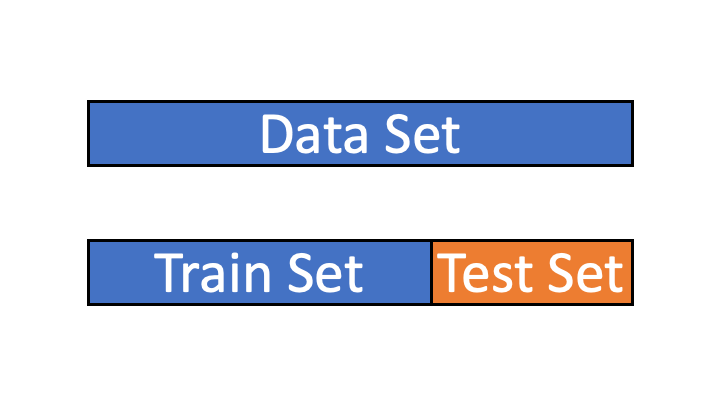
\includegraphics[width=\textwidth]{figures/ppt/TrainTestSplit.png}
    \caption{
      This figure shows how a data set can be partitioned for a supervised machine learning paradigm. The "data-set" is partitioned into two unequal sets with the "Train Set" having more data assigned to it than the "Test Set".  The "Train Set" and "Test Set" ratios can vary and is typically determined by the practitioner. There are many ways to partition the data for the train and test sets. For example the dataset can be partitioned sequentially from the data, or form partitions based on the data being randomly sampled.
      }
\label{fig:TrainTestSplit}

  \end{figure*}


\begin{figure*}[!htb]
    \centering
      \centering
      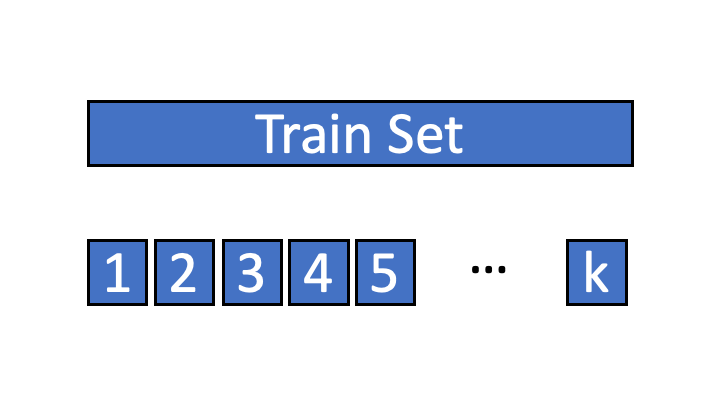
\includegraphics[width=\textwidth]{figures/ppt/KFoldValidation.png}
    \caption{
	The "Train Set" here represents the "Train Set" in Figure \ref{fig:TrainTestSplit}. In this figure the data is split into \(k\) folds. How the \(k\) folds are created can vary. A common technique is to randomly divide the "Train Set" observations into \(k\) equal folds.
      }
     \label{fig:KFoldValidation}
  \end{figure*}

\begin{figure*}[!htb]
    \centering
      \centering
      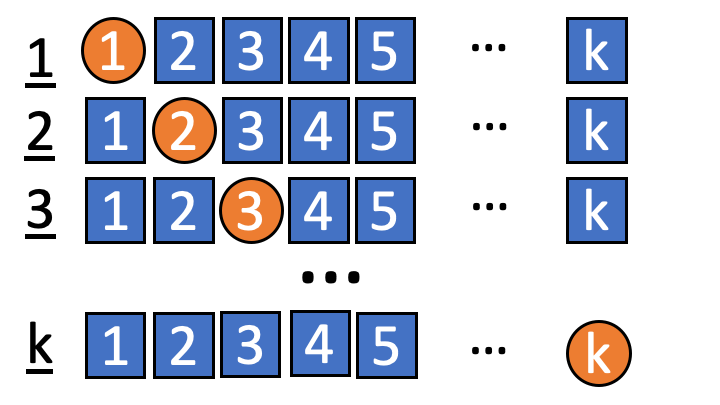
\includegraphics[width=\textwidth]{figures/ppt/KFoldValidationExplain.png}
     
    
    \caption{
	This figure breaks down how \(k\)-Fold Cross Validation works. These folds are created from "Train Set" in Figure \ref{fig:KFoldValidation}. For the first iteration (where you see 1 underlined), the first fold (circle labeled 1) is used to assess the models ability and the remaining folds (squares) are used to train the model. The second iteration follows the same procedure as the first except only the second fold is withheld and the other folds are used. This repeats \(k\) times.
      }
\label{fig:KFoldValidationExplain}
  \end{figure*}

\begin{figure*}[!htb]
    \centering
      \centering
      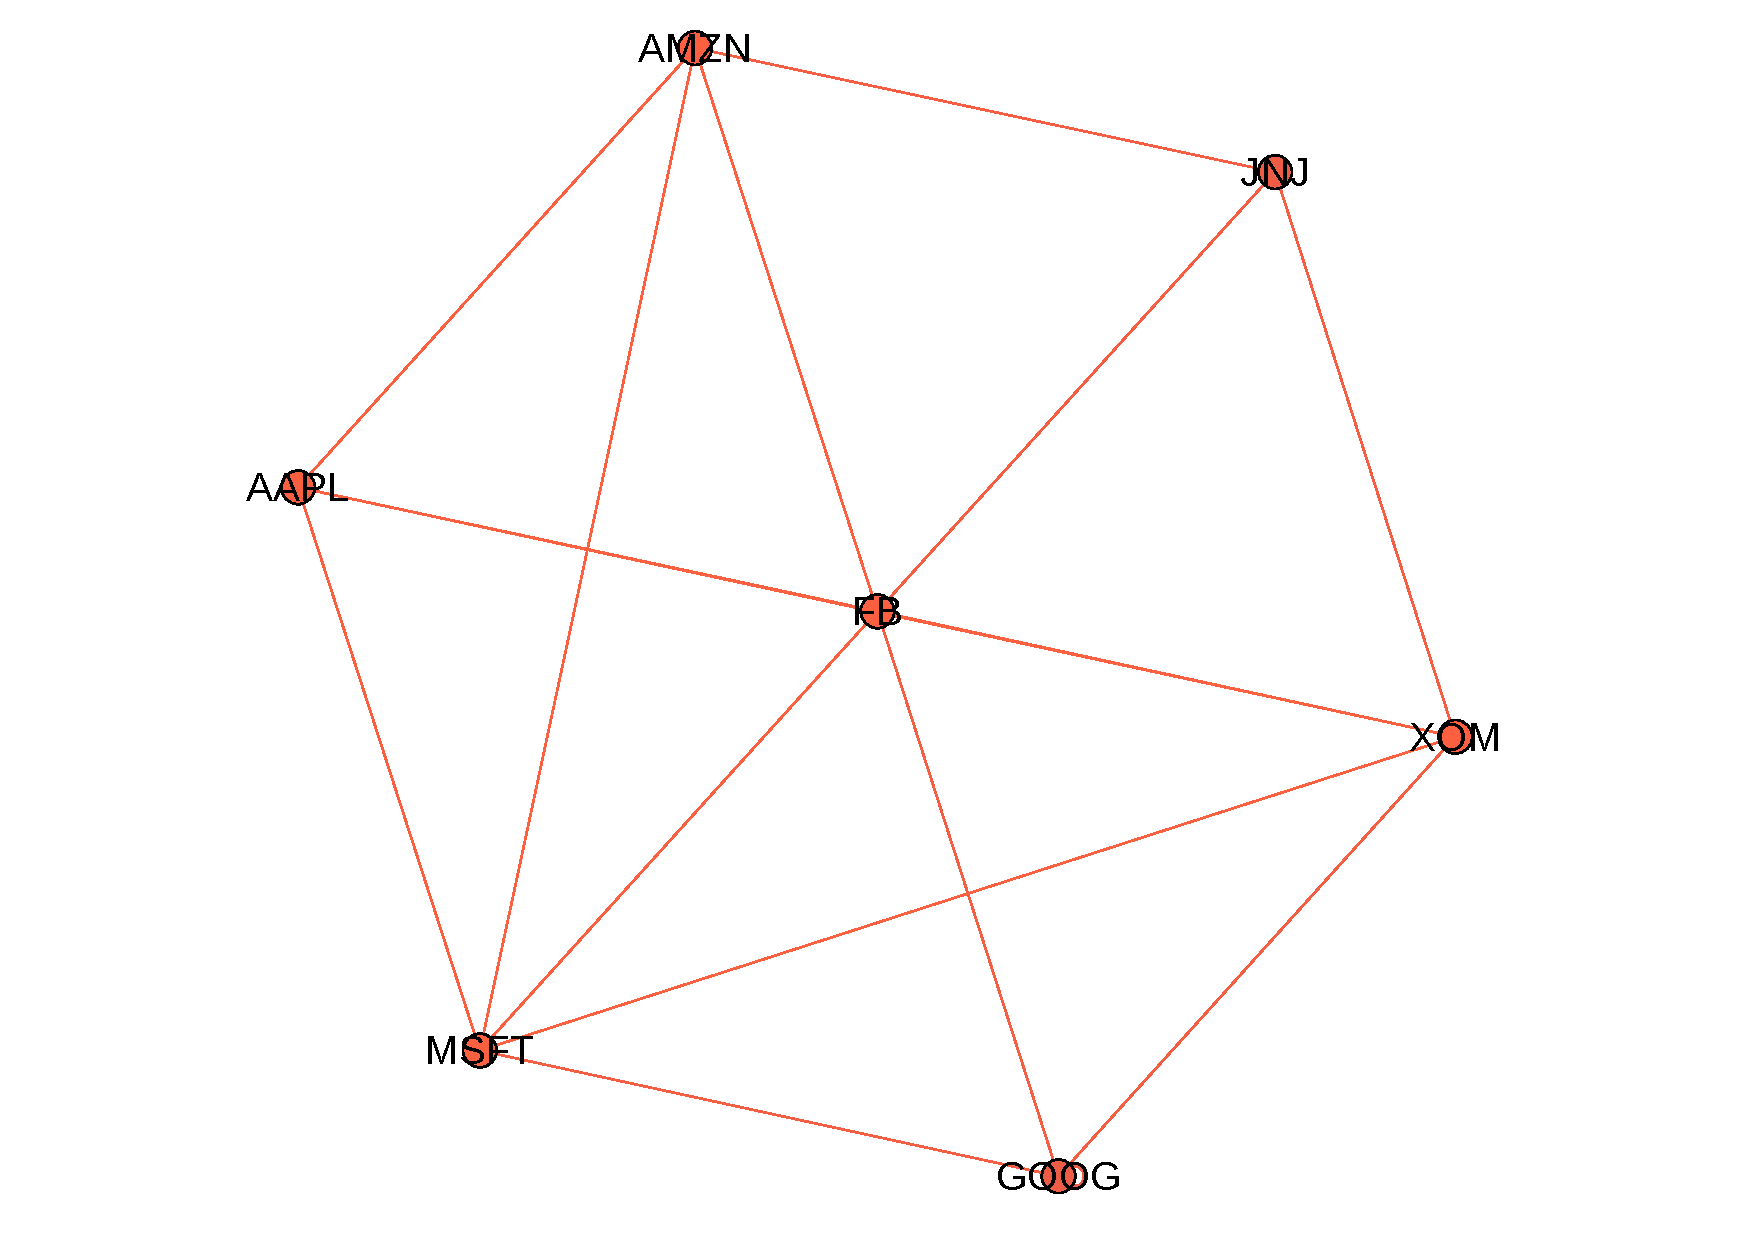
\includegraphics[width=\textwidth]{figures/Intro/ExampleNetwork.pdf}

      \caption{
      This figure contains an example of an undirected graph with seven nodes and sixteen edges. This graph is formed from randomly selecting stock symbol tickers from a set of tickers and forming connections randomly. The purpose of this data is solely to demonstrate the basics of network theory. The nodes are defined as circles and have ticker symbols overlaid on them. Edges are formed between nodes with lines between them.  Since this is an undirected graph there is no directional information or no distinction as to whether one node is connected to another or vice-versa.  The only information represented from an undirected graph is that they are connected.  
      }
      \label{fig:IntroExampleNetwork}

  \end{figure*}

%\RC{In general; I was trained to write out numbers less than one hundred. I made some changes, if you concur, maybe do so globally}

\begin{figure*}[!htb]
    \centering
     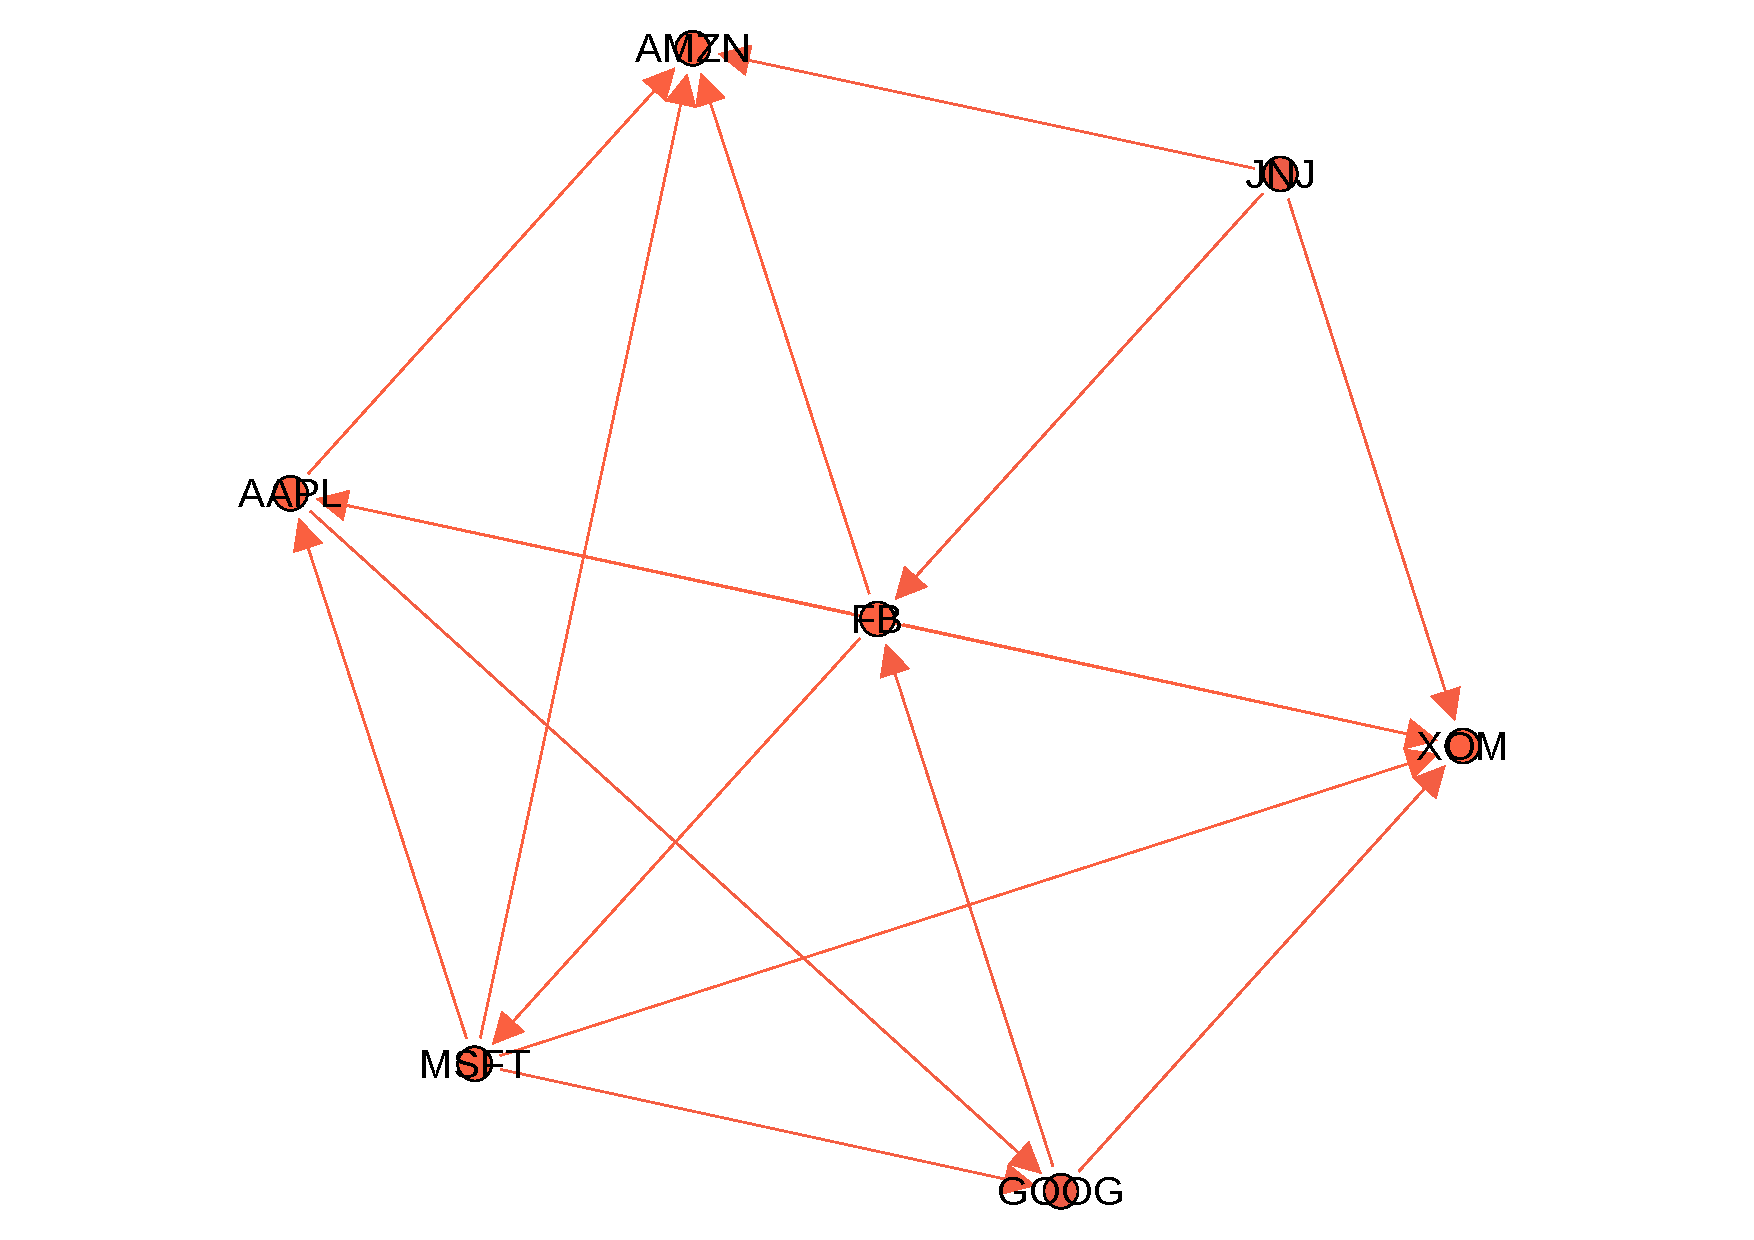
\includegraphics[width=\textwidth]{figures/Intro/ExampleNetworkDirected.pdf}
    \caption{
This graph is nearly identical to the graph in Figure \ref{fig:IntroExampleNetwork} except this graph is a directed network. This means that it contains directional information between the nodes. This directional information is communicated based on the position of the arrow in a line. For example, the node \(FB\) has an edge to \(MSFT\) however \(MSFT\) does not have an edge to \(FB\). The directional information allows other metrics to be used such as in-degree (which represents the amount of edges directed toward a node) and out-degree (which represents the amount of edges directed away from a node. In this example \(FB\) has an in-degree of two, an out-degree of four and a degree of six.
      }
	\label{fig:ExampleNetworkDirected}
\end{figure*}



  \begin{figure*}[!htb]
    \centering
      \centering
      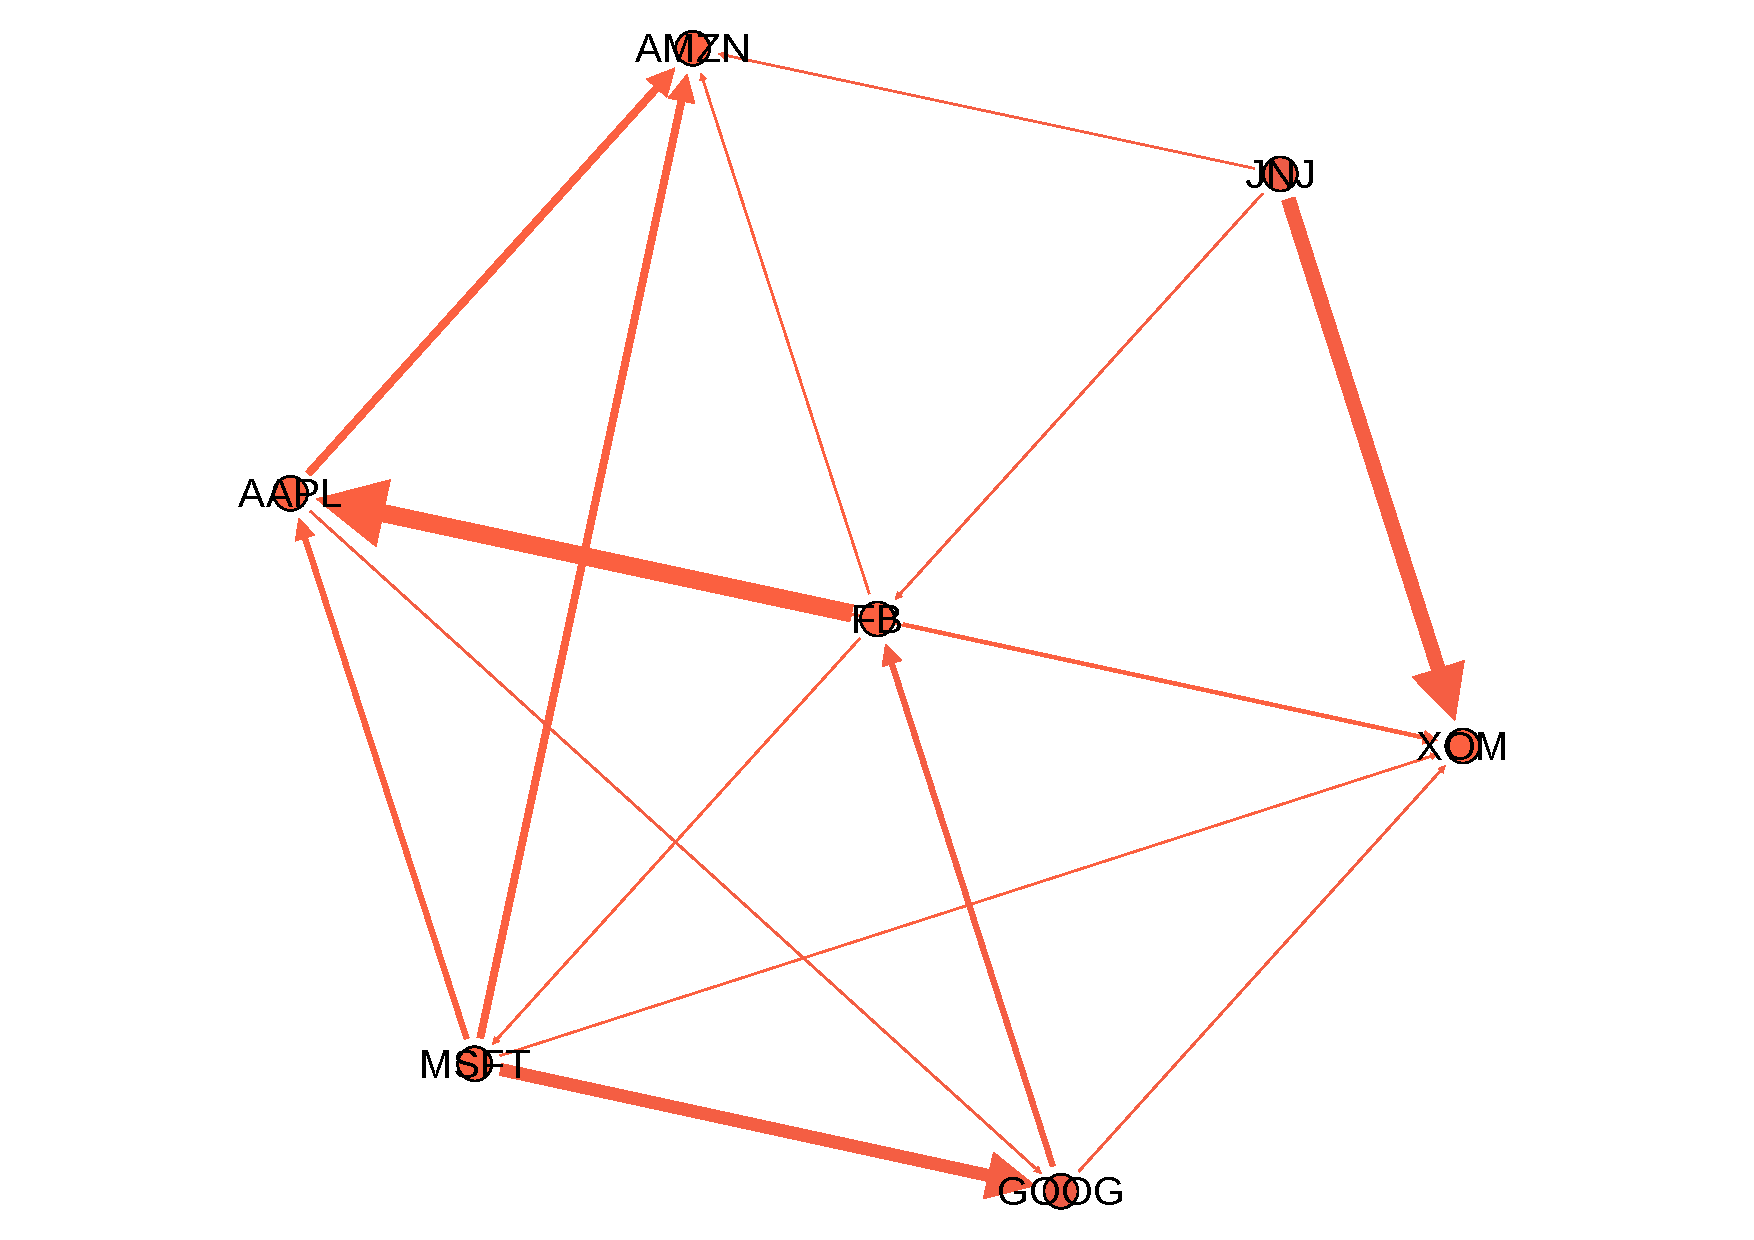
\includegraphics[width=\textwidth]{figures/Intro/ExampleNetworkDirectedWeighted.pdf}
      \caption{A nearly identical graph to the graph in Figure \ref{fig:ExampleNetworkDirected}. This directed graph contains weighted edges where a thick edge represents a high weight value (or strong connection). The smaller the edge weight value the thinner the edge will be.  Here \(FB\) has a strong connection to \(AAPL\) whereas \(FB\) has a weak connection to \(AMZN\).}
      \label{fig:ExampleNetworkDirectedWeighted}
    
  \end{figure*}

\begin{figure*}[!htb]
    \centering
      \centering
      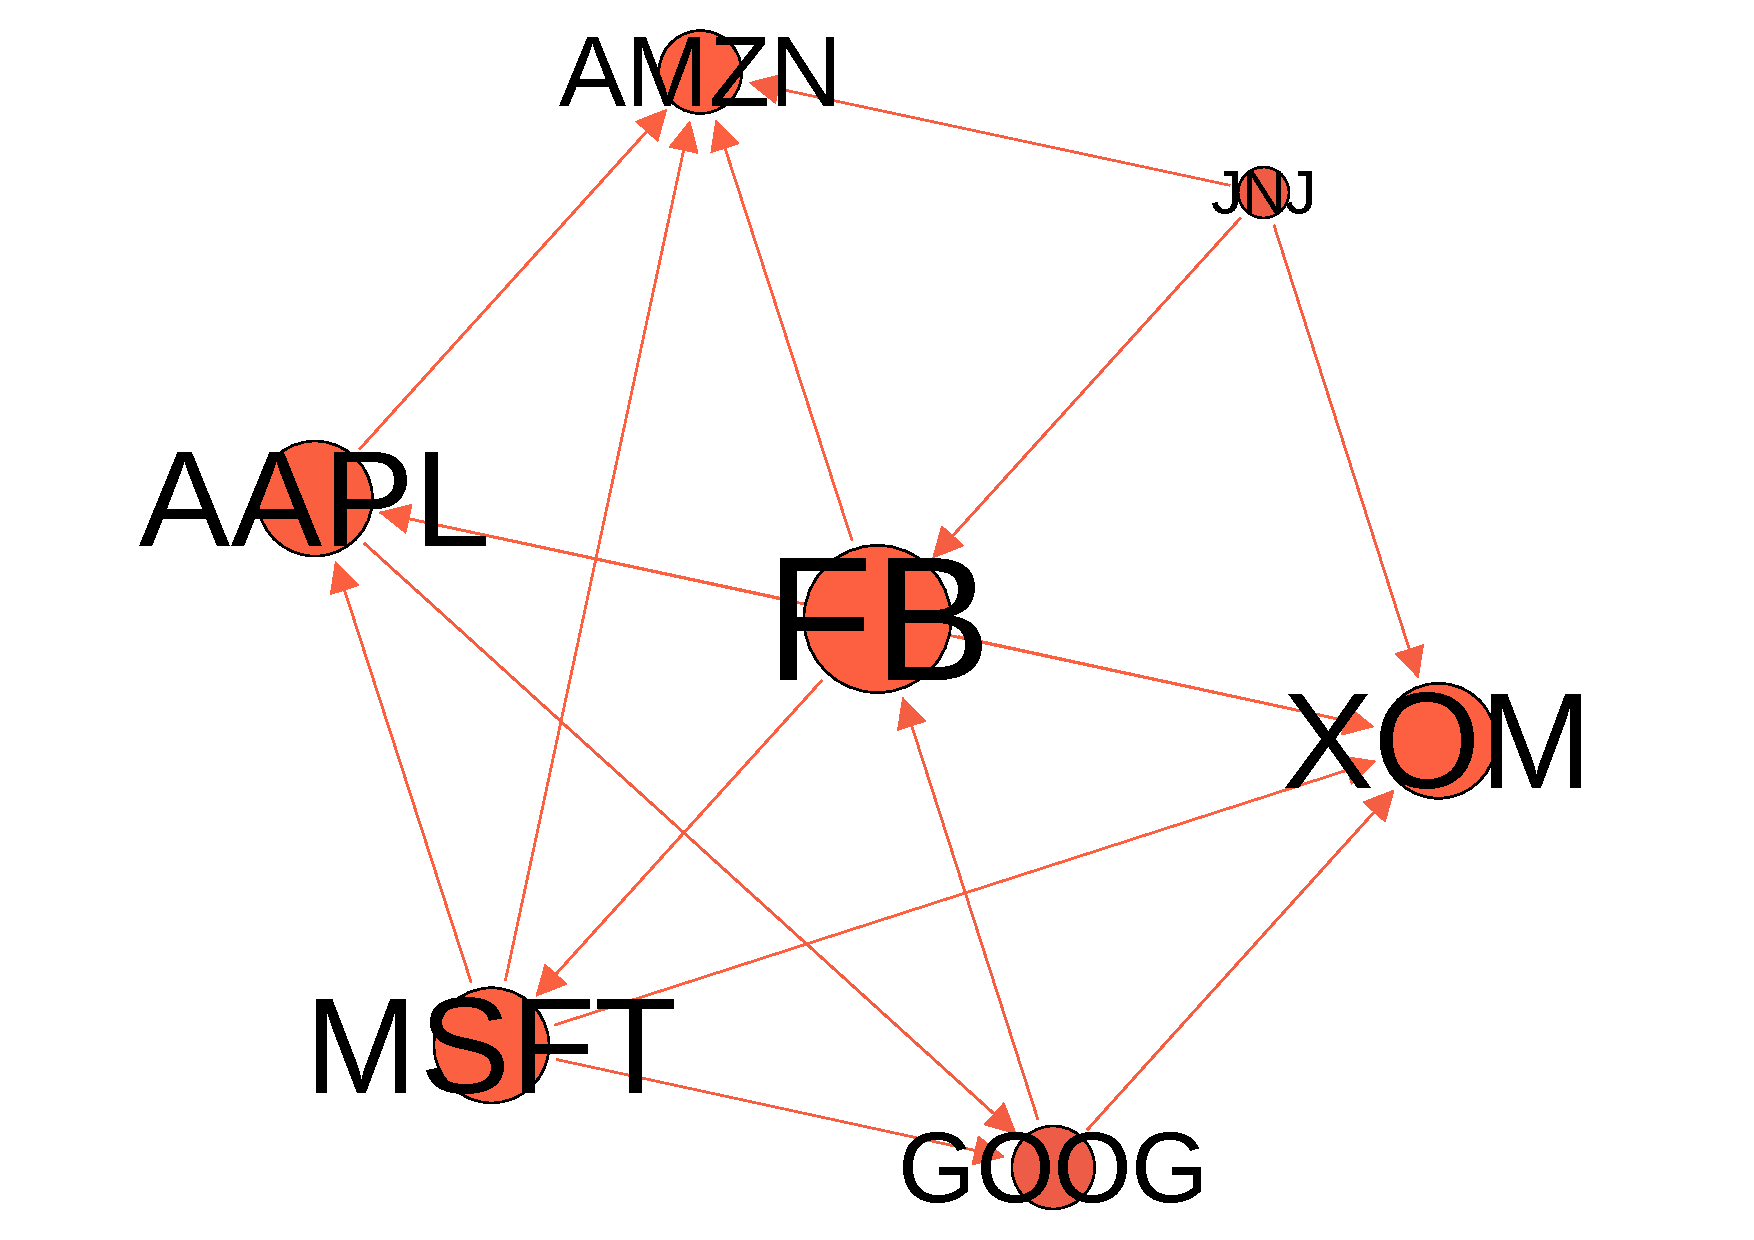
\includegraphics[width=\textwidth]{figures/Intro/ExampleNetworkDegree.pdf}
    \caption{
      A nearly identical graph to the graph in Figure \ref{fig:ExampleNetworkDirected}. Here the node sizes are scaled based on the degree. The higher the degree the larger the node size and consequently the smaller the degree the smaller the node size.
      }
      \label{fig:ExampleNetworkDegree}
  \end{figure*}






\clearpage

\begin{table}[htbp]
\begin{center}
    \begin{tabular}{|p{2cm}|p{1.5cm}|p{1.5cm}|p{1.5cm}|p{1.5cm}|p{1.5cm}|p{1.5cm}|p{1.5cm}|  }
        \hline
         & MSFT & AAPL & AMZN & FB & JNJ &  GOOG & XOM\\
        \hline
        MSFT  & 0 & 1 & 1 & 1  & 0 & 1 & 1 \\
        \hline
        AAPL & 1& 0 & 1 & 1 & 0 & 1 & 1 \\
        \hline
        AMZN & 1 & 1 & 0 & 1 & 1  & 0 & 0 \\
        \hline
        FB & 1 & 1 & 1 & 0  & 1 & 1 & 1 \\
        \hline
        JNJ & 0 & 0 & 1 & 1 & 0 & 0 & 0  \\ 
        \hline
        GOOG & 1 & 1 & 0 & 1 & 0 & 0 & 1 \\
        \hline
        XOM & 1 & 1 & 0 & 1 & 0 & 1 & 0  \\
        \hline
    \end{tabular}
\end{center}
\caption{ 
      This table contains an example of simulated data. This table was formed from randomly selecting stock symbol tickers from a set of tickers. The purpose of this data is solely to demonstrate the basics of network theory. Here the columns and row indicies belong to the selected tickers. The values contain either a one to represent if there is a connection between the ticker at a particular row index \(i\)  and the ticker of a particular column \(j\) or a zero if there is no connection.
}

\label{tab:ExampleTable}
\end{table}


%\clearpage
%\bibliographystyle{plainnat}
%\bibliography{thesisbib}

\bibliographystyle{plainnat}
\nobibliography{thesisbib}